\subsection{Annexes}
\subsubsection{Organigramme de l'IFSEM}
\centerline{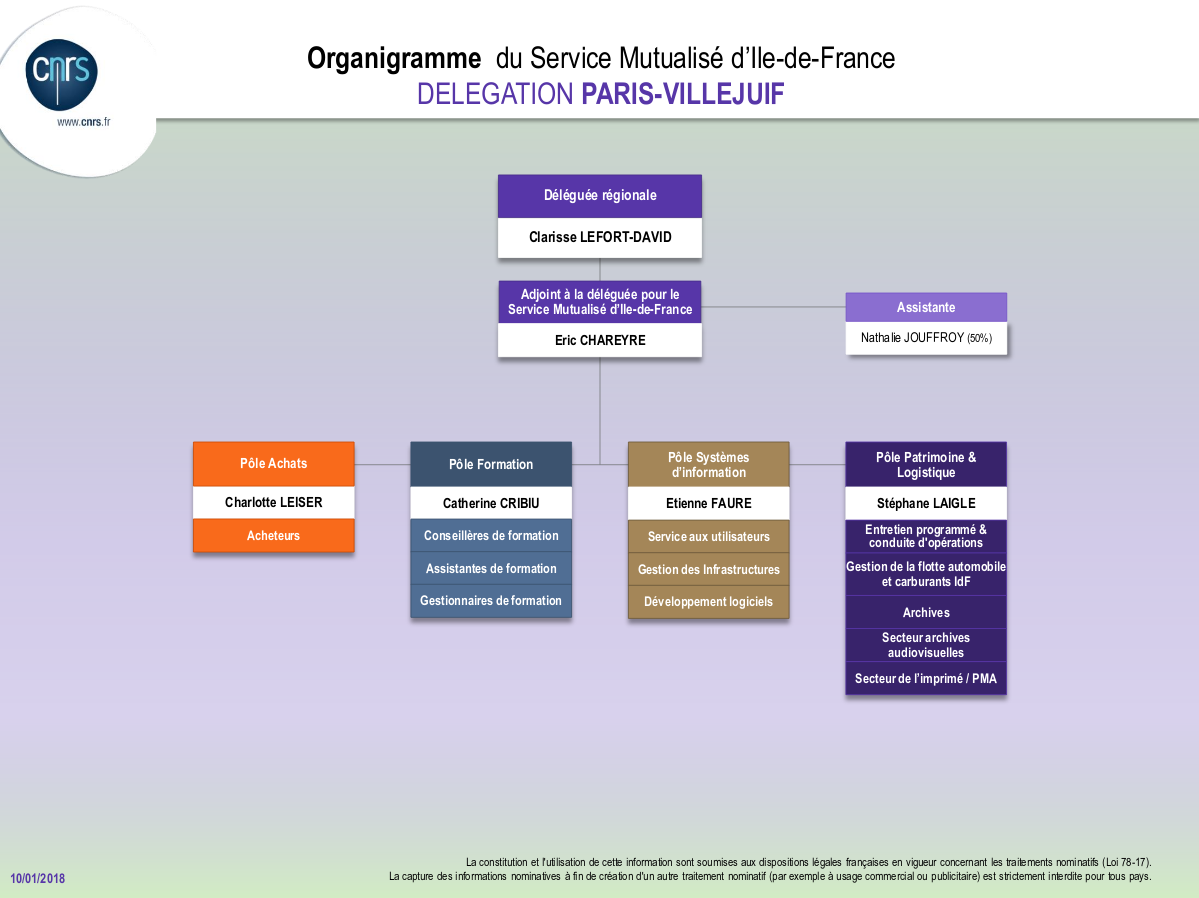
\includegraphics[width=15cm]{./images/ifsemorga.png}}

\subsection{Sources}
\begin{itemize}
    \item \url{http://www.cnrs.fr/}
    \item \url{https://www.dr1.cnrs.fr/spip.php?rubrique59}
    \item \url{https://fr.wikipedia.org/wiki/Centre_national_de_la_recherche_scientifique}
    \item \url{https://otrs.com/product-otrs/}
    \item \url{https://www.dr1.cnrs.fr/spip.php?article180}
    \item \url{https://blog.misterbean.fr/machine-cafe-entreprise}
    \item \url{https://www.quest.com/fr-fr/products/kace-systems-management-appliance/}
\end{itemize}
\newpage
\subsection{Attestation de fin de stage}
\newpage
\subsection{Ordre de mission}
Comme expliqué en partie 3.1.2, j'ai du me déplacer sur le campus de Meudon. J'ai donc fait faire une demande d'ordre de mission sans frais. Voici ladite demande :
\\
\\
\textit{
Bonjour,\\
Je soussigné Etienne FAURE, responsable du pôle SI de l’IFSeM, atteste que Théo \\PERESSE-GOURBIL actuellement stagiaire de 1ere année de l’ESIEE Paris effectuera un déplacement professionnel à la délégation Régionale du CNRS à Meudon (92) le jeudi 18 juillet 2019 pour la journée.
\medbreak
Pour faire valoir ce que de droit.
\smallbreak
Etienne FAURE}
\subsection{Remerciement}